%%%%%%%%%%%%%%%%%%%%%%%%%%%%%%%%
\section{The WA105 Dual-Phase Demonstrator}
\label{sec:proto-cern-double}

In recent years, two consecutive FP7 Design Studies
(LAGUNA/LAGUNA-LBNO) have led to the development of a conceptual
design (fully engineered and costed) for a 20-kt/50-kt GLACIER-type
underground neutrino detector. In these studies, an underground
implementation has been assumed {\textit{ab initio} 
and such constraints have been important and taken into account in
design choices. The LAGUNA-LBNO design study, completed in August
2014, has produced many technnical developments focused on the
construction of large and affordable liquid argon underground
detectors addressing the complete investigation of three-flavor
neutrino oscillations and the determination of their still unknown
parameters.
%
These detectors will be very powerful for non-beam studies as well,
such as proton decay, atmospheric neutrinos and supernova neutrinos.

The WA105 experiment is designed to provide a full-scale demonstration
of these technological developments. It will be exposed to a beam of
charged hadrons/electrons/muons of 0.5--20~GeV/c to characterize the
detector response to hadronic and electromagnetic showers.  A detailed
description of the experiment is available in the Technical Design
Report of 2014~\cite{WA105_TDR} and an up-to-date picture of
technical developments can be found in the Status Report\cite{WA105_SREP}
submitted to the SPSC CERN committee in March
2015. These developments form the basis of the
Alternative Far Detector design for DUNE, described in
Chapter~\ref{ch:detectors-fd-alt}.


The WA105 demonstrator is a dual-phase LArTPC with an active volume of
6$\times$6$\times$6~m$^3$.
%\fixme{why not quote fiducial?} 
These dimensions are motivated by the 4$\times$4~m$^2$ Charge Readout
Plane (CRP) units that are the basic readout components of the
large-scale LAGUNA/LBNO 20--50-kt detectors.
%
The 6$\times$6$\times$6~m$^3$ active volume is consistent with a fiducial
volume that accommodates the CRP size and provides full containment of
hadronic showers.
%
Surface operation prohibits drift lengths above 6~m. The footprint of
the active volume corresponds to 1:20 of the surface of the LBNO 20-kt
detector. The active volume contains about 300 tons of LAr. The
important parameters of the detector are presented in
Table~\ref{tab:demo_para} and Figures~\ref{fig:6by6_open}~\ref{fig:6by6_plan}
and~\ref{fig:6by6_vert} provide a 3D drawing and two cut views.
\begin{cdrtable}[Parameters for the WA105 Demonstrator]{lcc}{demo_para}{Parameters for the WA105 Demonstrator}
Liquid argon density & T/m$^3$& 1.38 \\ \toprowrule
Liquid argon volume height & m& 7.6 \\ \colhline
Active liquid argon height& m  & 5.99 \\ \colhline
Hydrostatic pressure at the bottom& bar & 1.03 \\ \colhline
Inner vessel size (WxLxH) &m$^3$ & 8.3 $\times$ 8.3 $\times$ 8.1\\ \colhline
Inner vessel base surface& m$^2$& 67.6 \\ \colhline
Total liquid argon volume& m$^3$ & 509.6 \\ \colhline
Total liquid argon mass & t & 705 \\ \colhline
Active LAr area & m$^2$& 36 \\ \colhline
Charge readout module (0.5 x0.5 m$^2$) & & 36\\ \colhline
N of signal feedthrough & & 12 \\ \colhline
N of readout channels & & 7680\\ \colhline
N of PMT & & 36 \\
\end{cdrtable}
\begin{cdrfigure}[Illustration of the  6$\times$6$\times$6~m$^3$  with the inner detector inside the cryostat]{6by6_open}{Illustration of the  $6\times 6\times 6$ $m^3$  demonstrator with the
detector inside the cryostat}
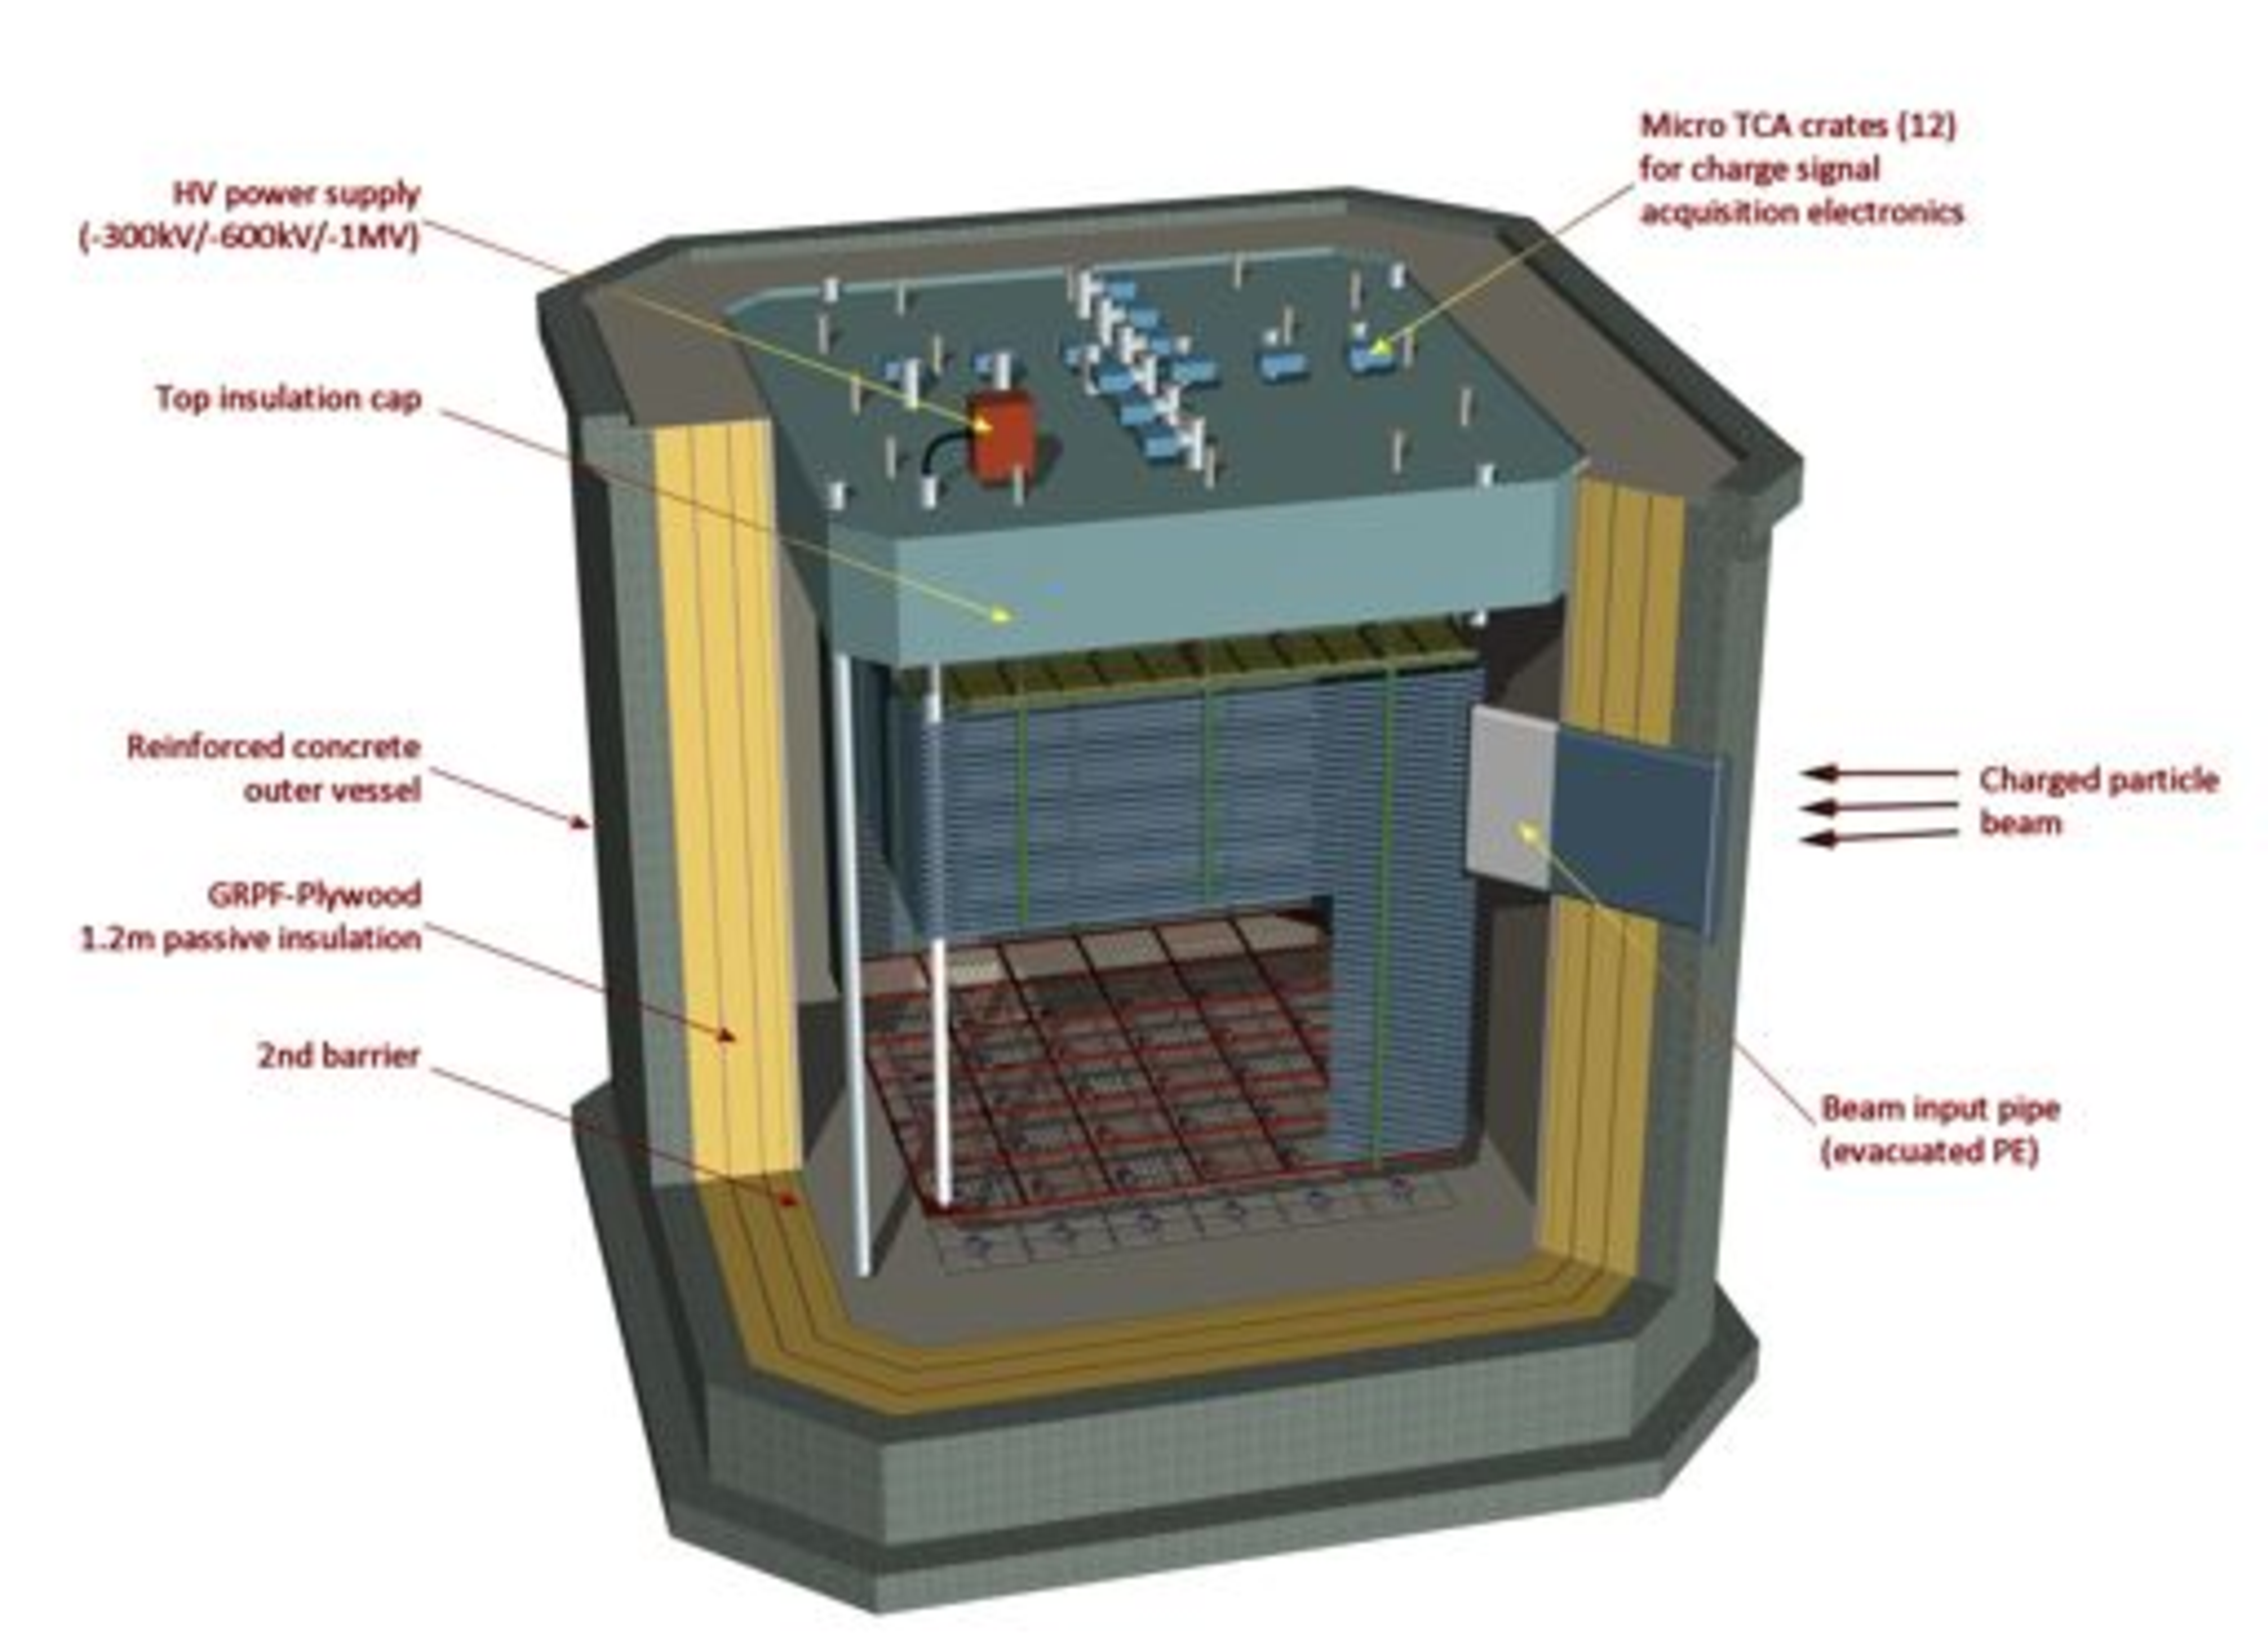
\includegraphics[width=0.8\linewidth]{130618_6x6x6m303v2}
\end{cdrfigure}
\begin{cdrfigure}[Plan view section of the $6\times 6\times 6$ $m^3$ demonstrator]{6by6_plan}{\small Plan view section of the $6\times 6\times 6$ $m^3$ demonstrator}
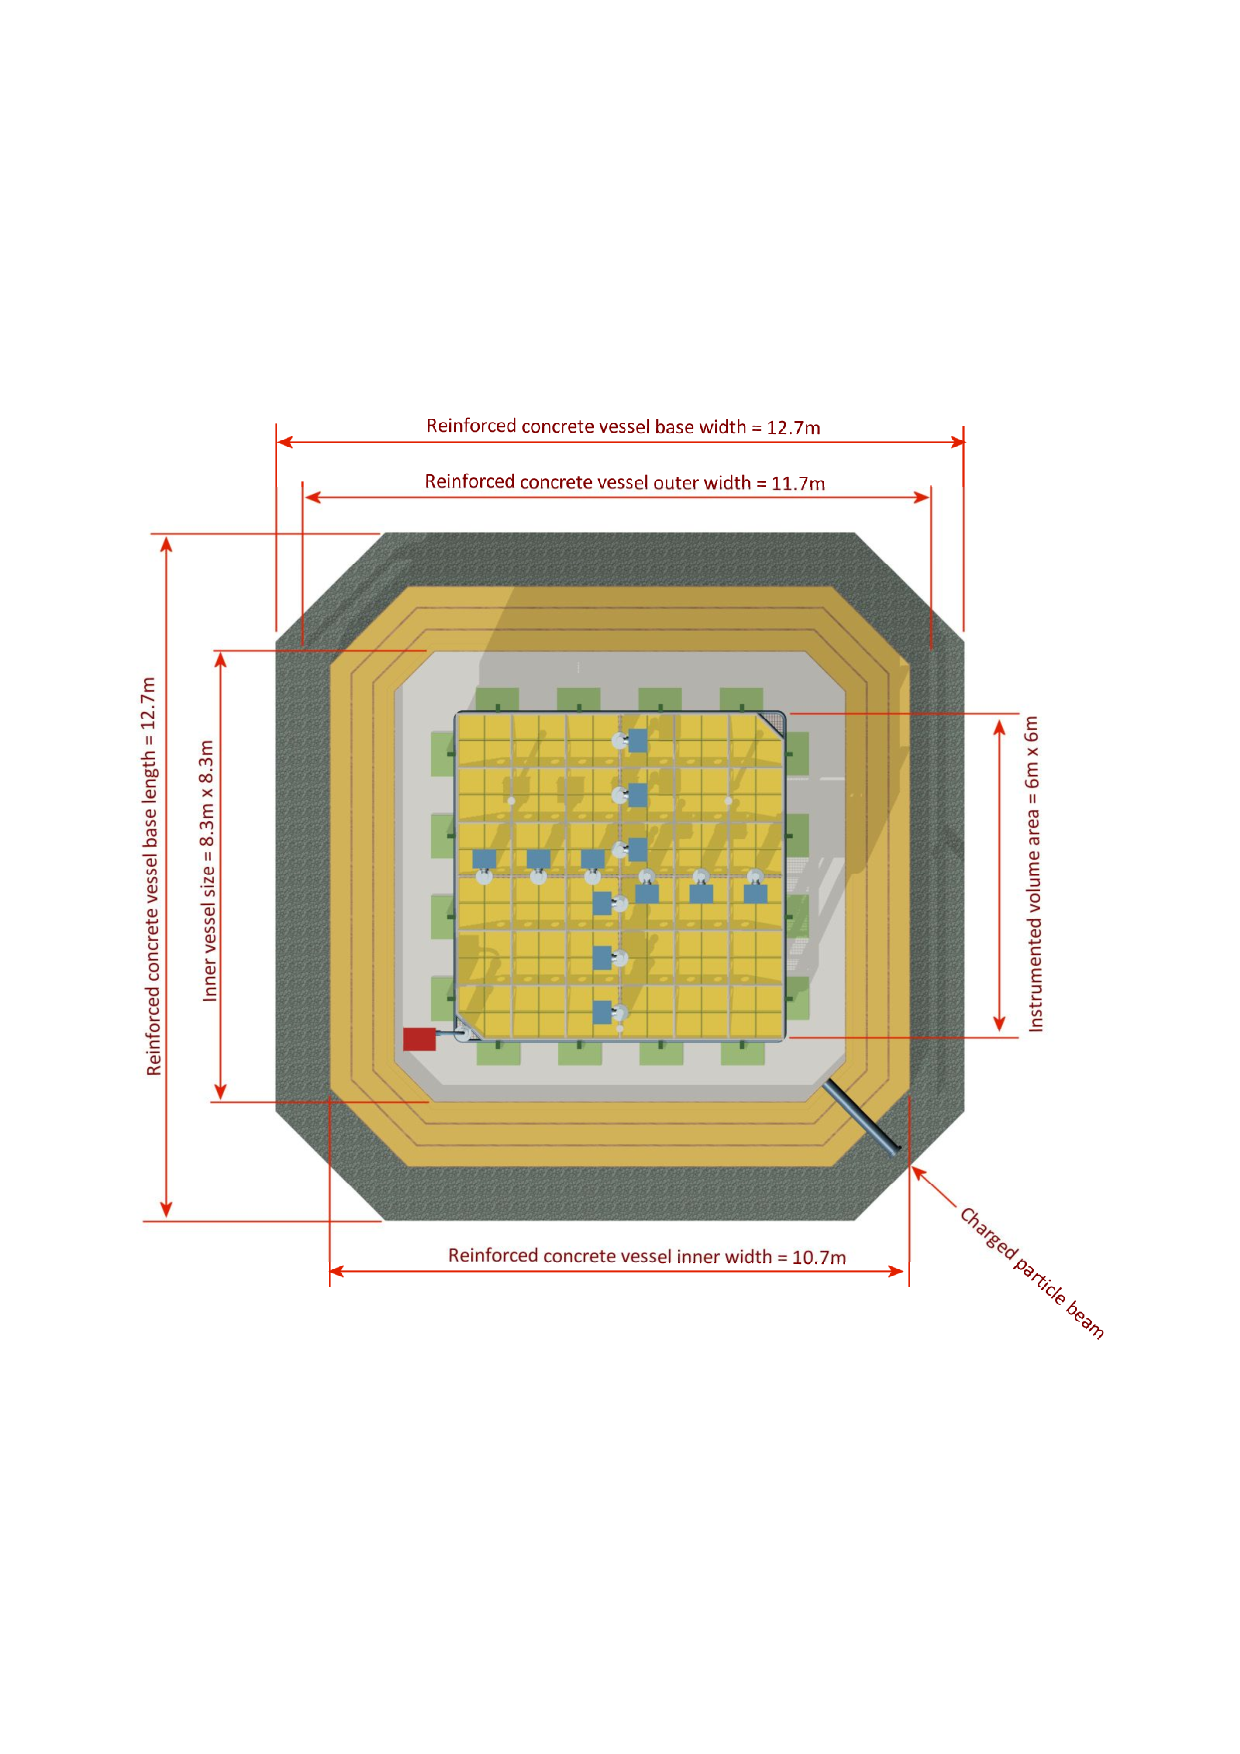
\includegraphics[width=0.7\linewidth]{Detector_overview_horizcross}
\end{cdrfigure}
\begin{cdrfigure}[\small Vertical cross section of the $6\times 6\times 6$ $m^3$ demonstrator]{6by6_vert}{\small Vertical cross section of the $6\times 6\times 6$ $m^3$ demonstrator}
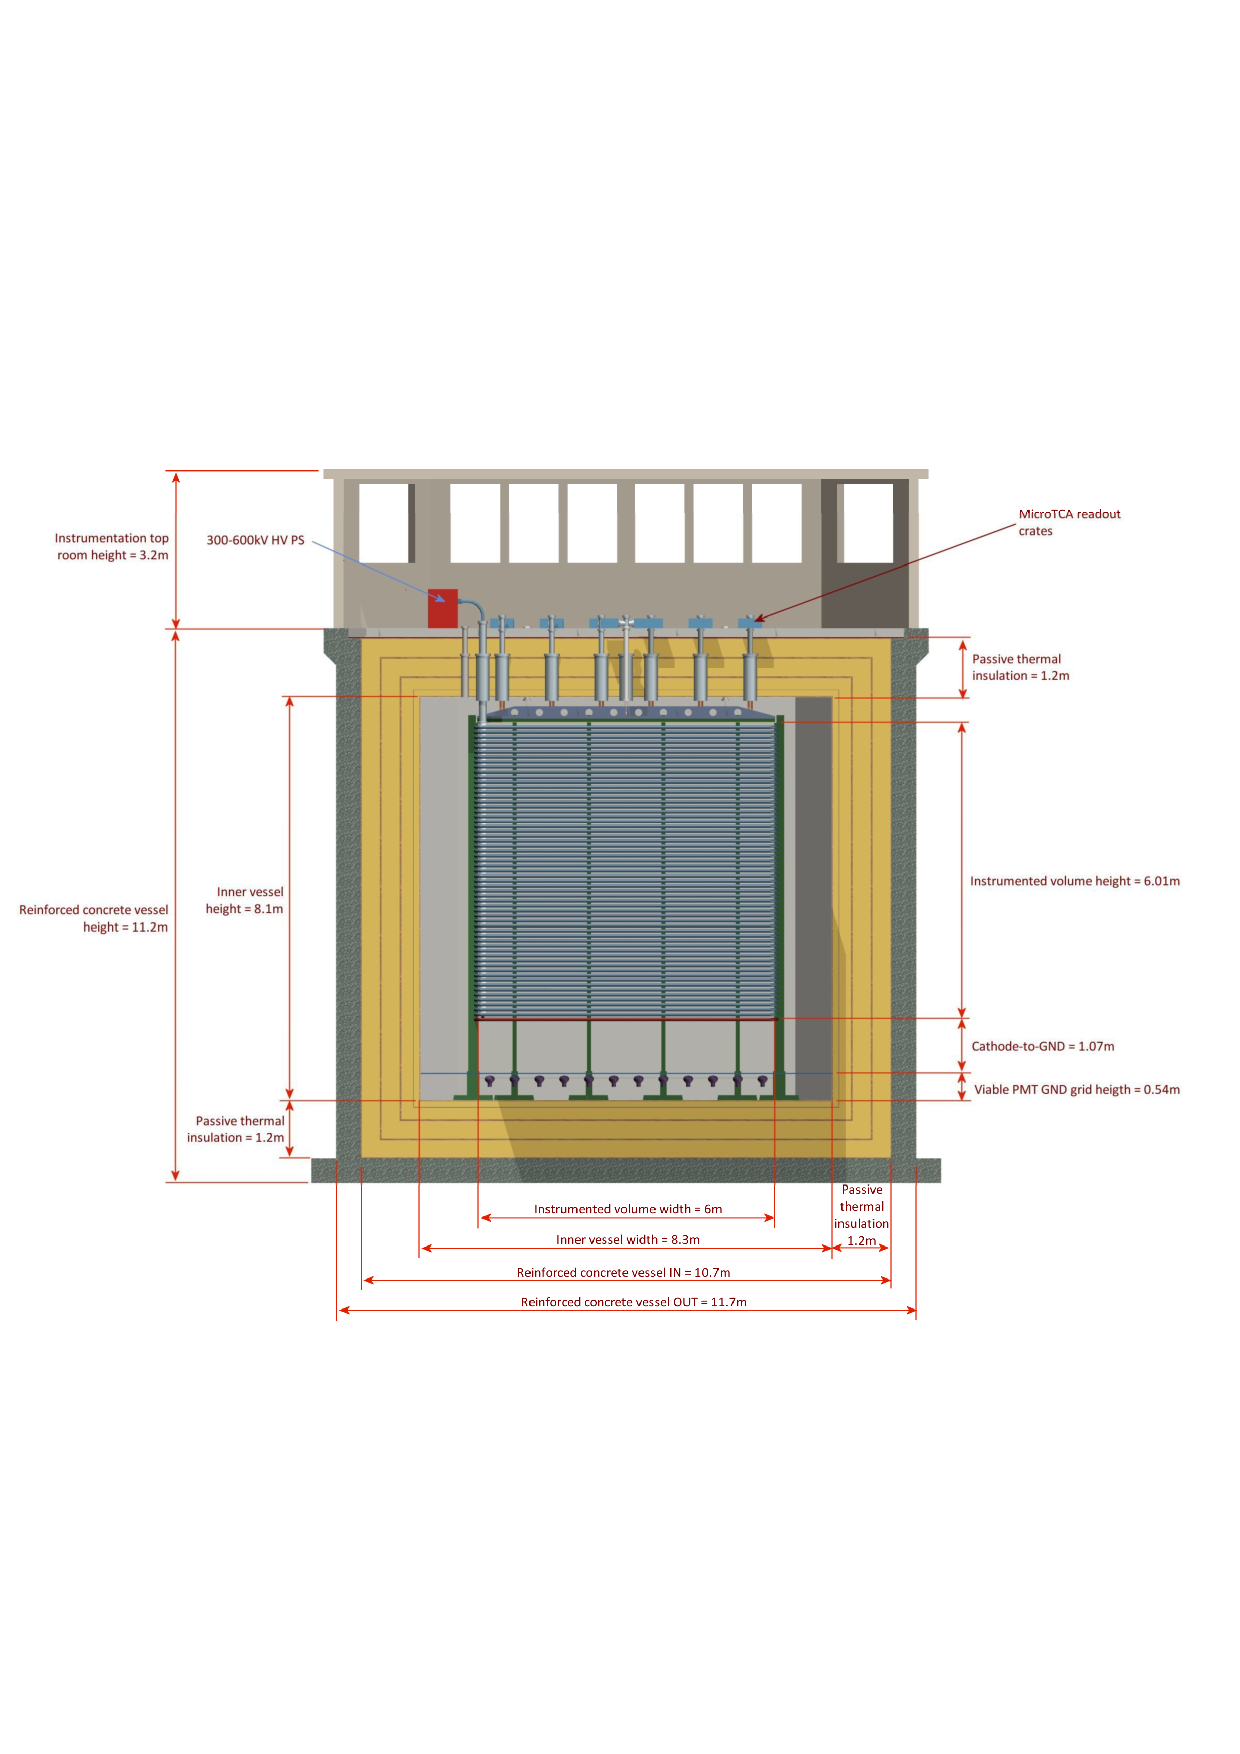
\includegraphics[width=0.7\linewidth]{Detector_overview_verticalcross}
\end{cdrfigure}


The dual-phase LArTPC design drifts ionization electrons
vertically through the LAr in a uniform electric field up to the
liquid-vapor interface, where they are extracted from the liquid into
the gas phase (GAr).
% by a higher field provided by a submersed grid.
In the GAr, the Charge Readout Plane (CRP) described in
Section~\ref{sec:detectors-fd-alt-chg-readout}, 
extracts, multiplies and collects the charge. 
%
The drift path in the WA105 demonstrator reaches 6~m with a drift
field of 0.5--1~kV/cm, corresponding to a cathode voltage of
$-$300--600~kV. The CRP has an active surface of 36 $m^2$, subdivided
into strips of 3.125-mm pitch and 3-m length, for a total of
\num{7680} readout channels.

%In the GAr, the electrons are then amplified %in the GAr thanks to avalanches occurring in micro-pattern detector called LEM (Large Electron Multiplier) and collected on a 2D anode made withe a printed circuit board. The sandwich structure composed by the LEM the Anode and the extraction grid is the so called Charge Readout Plane. The gain provided by the amplification in gas allows for the compensation of the charge attenuation along long drift paths and to achieve a S/N greater than 100 for minimum ionizing particles over 12m drift path.The drift path in the WA105 demonstrator reaches 6 m, the detector is foreseen to work with a drift field of 0.5 kV/cm and 1 kV/cm, corresponding to a voltage applied to the cathode respectively of -300kV and -600 kV. The CRP has an active surface of 36 $m^2$ subdivided in strips of 3.125 mm pitch and 3 m length for a total of 7680 readout channels.

The WA105 demonstrator will demonstrate the techniques developed for
the 20/50-kt LBNO detectors, in particular:
\begin{itemize}
\item{tank construction technique based on the LNG industry with non-evacuated vessel}
\item{purification system}
\item{long drift}
\item{HV system 300--600~kV, large hanging field cage}
\item{large area double-phase charge readout}
\item{accessible cryogenic front-end electronics and cheap DAQ electronics}
\item{long-term stability of UV light readout}
\end{itemize}

Furthermore, the 6$\times$6$\times$6~m$^3$ demonstrator exposed to the
test beam promises a rich physics program of
\begin{itemize}
\item{assess detector performance in reconstructing hadronic showers; the most demanding task in neutrino interactions}
\item{measure hadronic and electromagnetic calorimetry and PID performance}
\item{full-scale software development, simulation and reconstruction}
\item{collect high-statistic hadronic interaction samples with unprecedented granularity and resolution for the study of hadronic interactions and nuclear effects}
\item{assess physics capabilities of the dual-phase versus
  single-phase performance, in particular: high S/N, 3-mm pitch,
  absence of materials in long drift space, two collection views, no
  ambiguities}
\item{study systematics related to
  the reconstruction of the hadronic system (resolution and energy
  scale), electron-identification efficiencies and $\pi^0$ rejection and particle $dE/dx$ identification for proton decay}
\end{itemize}



The 6$\times$6$\times$6~m$^3$ WA105 detector is expected to start data
taking in 2018 in the EHN1 Hall extension currently under
construction at CERN.  The detector components are in an advanced
state of design/prototyping, or preproduction. 
Completion of the WA105 detector design and the
preparation of its construction have been progressing very quickly.
Many technical design details are benefitting from the
implementation of a 20-t (3$\times$3$\times$1~m$^3$) prototype (see Figure~\ref{fig:3by1}),
which is the minimal size
of a readout unit in the final far detector.  
\begin{cdrfigure}[Exploded view of the  3$\times$3$\times$1~m$^3$  prototype]{3by1}{Exploded view of the 3$\times$3$\times$1~m$^3$  prototype}
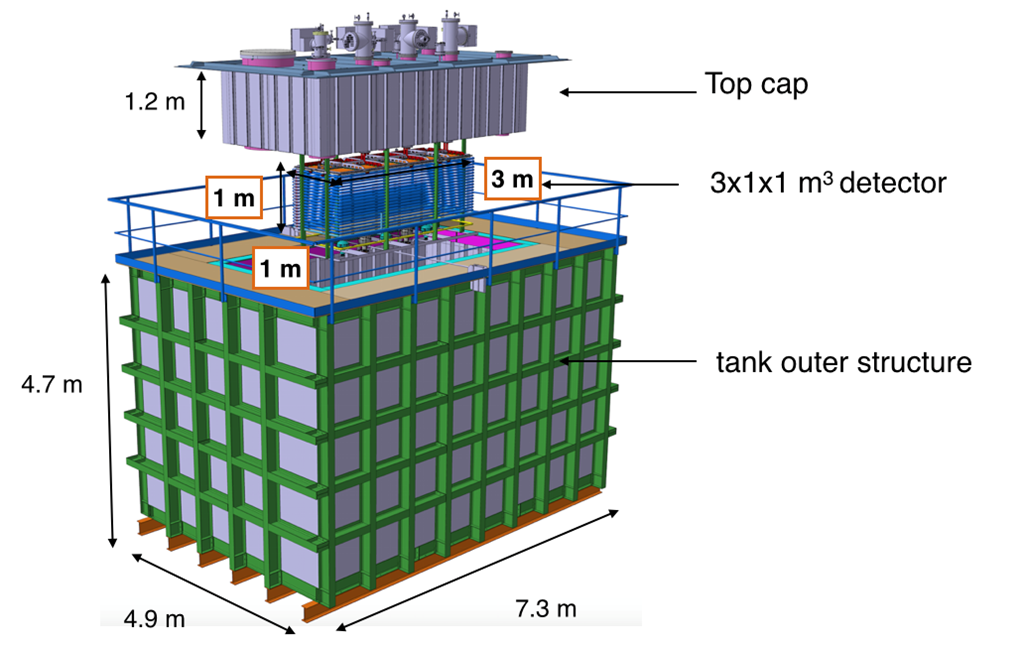
\includegraphics[width=0.95\linewidth]{3by1}
\end{cdrfigure} 
Development of this 20-t prototype has verified
the complete system integration: 
production of fully engineered prototype versions of many detector
parts including installation details and ancillary services;
establishment of the Quality Assessment (QA) procedures for the
construction, installation and commissioning chains; establishment of
the procurement processes for the major detector components; and
validation of the cost and schedule estimates for WA105.  The
3$\times$3$\times$1~m$^3$ 20-t prototype represents a technical test
bed and integration exercise to accelerate the design, procurement, QA
and commissioning activities needed for the 6$\times$6$\times$6-m$^3$
detector.  In particular, a complete procedure for construction of
GTT-licensed corrugated membrane cryostats 
been established at CERN and a full chain for the procurement,
processing, assembly and commissioning of the LEM detectors and 
anodes has been implemented.

